% Source - https://tex.stackexchange.com/a/498024
% Posted by user121799, modified by community. See post 'Timeline' for change history
% Retrieved 2026-04-19, License - CC BY-SA 4.0

% UMBC Colors: https://styleguide.umbc.edu/umbc-colors/
% Primary Colors
\definecolor{umbcgold}{RGB}{253,181,21}
\definecolor{black}{RGB}{0,0,0}
% Secondary Colors
\definecolor{umbcred}{RGB}{218,33,40}
\definecolor{umbclightgray}{RGB}{199,200,202}
\definecolor{umbcaokteal}{RGB}{0,113,118}
\definecolor{umbcretrieverbrown}{RGB}{166,122,5}
\definecolor{umbcdarkgray}{RGB}{99,100,102}

\usetikzlibrary{matrix}
\tikzset{
  payoff matrix/.style={
    matrix of nodes,
    column sep=-\pgflinewidth,
    row sep=-\pgflinewidth,
    nodes={
      text height=.75em,
      text width=7.5em,
      draw,
      path picture={
        \fill[umbcred!20] (path picture bounding box.north west) -|
          (path picture bounding box.south east);
        \fill[umbcaokteal!20] (path picture bounding box.north west) |-
          (path picture bounding box.south east);
      },
      labelrow/.style={
        path picture={
          \fill[umbcred!20] (path picture bounding box.south west)
                          rectangle (path picture bounding box.north east);
        }
      },
      labelcol/.style={
        path picture={
          \fill[umbcaokteal!20] (path picture bounding box.south west)
                          rectangle (path picture bounding box.north east);
        }
      }
    }
  }
}

\newcommand{\pft}[2]{
    {\hfill #1 \par
    #2 \hfill}
}

\begin{figure}
    \centering
    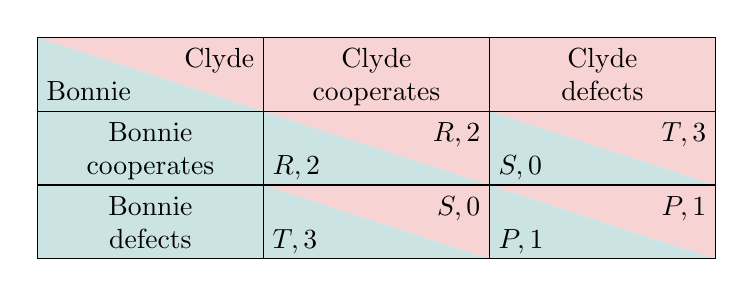
\begin{tikzpicture}[
        every node/.style={%
        align=center,
        anchor=center,
        text depth=1.25em,
      }
    ]
    \matrix [payoff matrix]{
    \pft{Clyde}{Bonnie}  & |[labelrow]| Clyde \par cooperates & |[labelrow]| Clyde \par defects \\
    |[labelcol]| Bonnie \par cooperates & \pft{$R,2$}{$R,2$} & \pft{$T,3$}{$S,0$} \\
    |[labelcol]| Bonnie \par defects & \pft{$S,0$}{$T,3$} & \pft{$P,1$}{$P,1$} \\
    };
    \end{tikzpicture}
    \caption{Payoff matrix for Bonnie and Clyde.}
    \label{fig:prisoners}
\end{figure}